% !TeX program = pdflatex
% =============================================================================
% Arbeitsblatt: Kondensatoren
% UZH Praktikum I -- Sara Romer Urban, Kantonsschule im Lee, HS2026
% Klassen: 4fh (regulaer, 25.08.2026) + 4cdeg (SP4, 28.08.2026) -- gemeinsames
% Material (siehe institutionen/UZH-Praktikum-I/CLAUDE.md, Abschnitt "SP
% (Schwerpunktfach) vs. regulaere Physik").
%
% Enthaelt Lernziele, Einleitung, alle Theorie-Abschnitte, die im Plenum
% behandelten Teile (Lehrervortrag, Demoversuch) sowie die Sortieraufgabe
% und die Herleitungs-Uebung zum Dielektrikum -- alles ausser der
% PhET-/Excel-Lernaufgabe. Diese steht (mit Excel-Vorlage) allein in
% aufgabenblatt3-kondensatoren-teil1.tex (Aufgaben, die eine Simulation
% oder Excel brauchen, gehoeren ins Aufgabenblatt); reine
% Vor-/Nachbereitungs-Uebungen in kondensatoren-zusatzaufgaben.tex.
%
% Quellen: lernziele.md (dieser Ordner), kondensatoren-notizen-sara-romer.txt
% (Besprechungsnotizen von Sara Romer), Vorwissen/Elektrostatik/ (Coulombkraft,
% E-Feld, Potential/Spannung -- bereits bekannt, hier nur repetiert), sowie die
% Referenzquellen direkt in diesem Ordner (LEIFIphysik, Physik Libre 12.11,
% HSHL "Lerninhalte und Abschlussarbeiten" -- von Letzterem nur die
% Wassereimer-Analogie und die qualitative Beschreibung, nicht die dortige
% Integral-/Ableitungsrechnung, die Hochschulstoff ist).
% =============================================================================
\documentclass[addpoints,11pt,a4paper]{exam}

\usepackage[T1]{fontenc}
\usepackage[utf8]{inputenc}
\usepackage[ngerman]{babel}
\usepackage{lmodern}
\usepackage[a4paper,margin=2.2cm,headheight=14pt]{geometry}
\usepackage{amsmath}
\usepackage{siunitx}
% Hausstil: zusammengesetzte Einheiten immer als echter Bruch (\frac), nicht
% als Inline-Schrägstrich oder \tfrac -- gilt global für jedes \si/\SI.
\sisetup{per-mode=fraction,fraction-command=\frac}
\usepackage{array,booktabs,tabularx,multirow}
\usepackage{enumitem}
\usepackage{xcolor}
\usepackage{colortbl}
\usepackage{tikz}
\usepackage{physics}
\usepackage{circuitikz}
\usepackage[most]{tcolorbox}
\usepackage{lastpage}
\usepackage{graphicx}
\usepackage{hyperref}

\usetikzlibrary{arrows.meta,calc,angles,quotes}

\usepackage{setspace}
\usepackage{needspace}
\setlength{\parindent}{0pt}
\setlength{\parskip}{0.6em}
\setstretch{1.08}
\setlist[itemize]{itemsep=0.4em}

% -----------------------------
% Farben (Corporate-Farbschema Physik KFR)
% -----------------------------
\definecolor{titleblue}{HTML}{183A6B}
\definecolor{accentblue}{HTML}{2E6F9E}
\definecolor{lightblue}{HTML}{EAF4FB}
\definecolor{verylightblue}{HTML}{F7FBFE}
\definecolor{lightgray}{HTML}{F4F6F8}
\definecolor{darkgray}{HTML}{4A4A4A}
\definecolor{accentorange}{HTML}{D9720C}
\definecolor{accentpurple}{HTML}{7B2D8E}
% Theorie-Block: eigene Farbe (grün).
\definecolor{theorygreen}{HTML}{2E7D4F}
\definecolor{lighttheorygreen}{HTML}{EAF7EF}
% Gruppenarbeit-Box: eigene Farbe (Petrol/Teal).
\definecolor{groupteal}{HTML}{1B7F72}
\definecolor{lightgroupteal}{HTML}{E8F5F3}
% Hinweisbox: Orange (accentorange), für wichtige Klarstellungen.
\definecolor{lightorange}{HTML}{FCEEE0}
% Formelbox: Violett (accentpurple), für die zentralen Formeln dieser Einheit.
\definecolor{lightpurple}{HTML}{F3EAF7}

% Links (hyperref): farblich ans Corporate-Farbschema angeglichen.
\hypersetup{
  colorlinks=true,
  urlcolor=accentblue,
  linkcolor=accentblue,
  pdftitle={Arbeitsblatt 4: Kondensatoren},
  pdfauthor={Loris Keller}
}

% -----------------------------
% Spaltentypen
% -----------------------------
\newcolumntype{Y}{>{\centering\arraybackslash}X}
\newcolumntype{P}[1]{>{\raggedright\arraybackslash}p{#1}}

% -----------------------------
% Boxen
% -----------------------------
\tcbset{before skip=10pt, after skip=10pt}
\newtcolorbox{titlebox}{
  enhanced,
  colback=titleblue,
  colframe=titleblue,
  boxrule=0pt,
  arc=3mm,
  left=3mm,right=3mm,top=3mm,bottom=3mm
}

\newlength{\aufgabenindent}
\settowidth{\aufgabenindent}{10.\hskip\labelsep}

% Praktikum I: Lernziele/Einleitung/Theorie/Aufgaben werden NICHT mehr
% farbig gerahmt (nur Formel-, Hinweis- und Antwortbox bleiben Boxen) --
% siehe institutionen/UZH-Praktikum-I/CLAUDE.md, Abschnitt "Boxen-Layout".
\newenvironment{infobox}{%
  \par\addvspace{10pt}\noindent
}{%
  \par\addvspace{10pt}
}

\newenvironment{theoriebox}[1][Theorie]{%
  \par\addvspace{10pt}\noindent\textbf{#1}\par\smallskip\noindent
}{%
  \par\addvspace{10pt}
}

% taskbox/groupbox stehen in questions VOR dem ersten \question (Bilder,
% Fliesstext) -- exam.cls' questions-Liste braucht dafür eine echte,
% eigenständige Box (sonst "Something's wrong--perhaps a missing \item",
% weil z.B. ein \begin{center} vor dem ersten \item der Aussenliste steht).
% Deshalb bleiben es tcolorboxen, nur unsichtbar gemacht (keine Farbe/Rahmen,
% kein Padding) statt sie durch reine Absätze zu ersetzen.
\newtcolorbox{taskbox}[1][]{
  enhanced, breakable,
  colback=white, colframe=white, boxrule=0pt,
  left=0mm,right=0mm,top=0mm,bottom=0mm,
  before skip=10pt, after skip=10pt,
  before upper={%
    \def\tmpboxtitle{#1}%
    \ifx\tmpboxtitle\empty\else\noindent\textbf{#1}\par\smallskip\fi
  }
}

\newtcolorbox{groupbox}[1][Gruppenarbeit]{
  enhanced, breakable,
  colback=white, colframe=white, boxrule=0pt,
  left=0mm,right=0mm,top=0mm,bottom=0mm,
  before skip=10pt, after skip=10pt,
  before upper={\noindent\textbf{#1}\par\smallskip}
}

% beispielbox: für die Einleitung und für durchgerechnete Beispiele
% innerhalb der Theorie -- wie die anderen Inhaltsboxen ungerahmt.
\newenvironment{beispielbox}[1][Beispiel]{%
  \par\addvspace{10pt}\noindent\textbf{#1}\par\smallskip\noindent
}{%
  \par\addvspace{10pt}
}

% hinweisbox: Orange, für wichtige Klarstellungen/Verwechslungswarnungen.
\newtcolorbox{hinweisbox}[1][Hinweis]{
  enhanced,
  breakable,
  colback=lightorange,
  colframe=accentorange,
  title={#1},
  fonttitle=\bfseries,
  boxrule=0.7pt,
  arc=2mm,
  left=5mm,right=5mm,top=2mm,bottom=2mm
}

% formelbox: Violett, um die zentralen Formeln dieser Einheit hervorzuheben.
\newtcolorbox{formelbox}[1][Formel]{
  enhanced,
  breakable,
  colback=lightpurple,
  colframe=accentpurple,
  title={#1},
  fonttitle=\bfseries,
  boxrule=0.9pt,
  arc=2mm,
  left=5mm,right=5mm,top=2mm,bottom=2mm
}

\newtcolorbox{answerbox}{
  breakable,
  colback=white,
  colframe=gray!55,
  boxrule=0.5pt,
  arc=1.5mm,
  left=2mm,right=2mm,top=2mm,bottom=2mm
}

% teilkopf: fette Zwischenüberschrift zur klaren Abgrenzung der Teile 1-4
% innerhalb der langen Lernaufgabe -- ungerahmt, wie die anderen
% Inhaltsboxen.
\newenvironment{teilkopf}{%
  \par\addvspace{8pt}\noindent\bfseries\sffamily
}{%
  \par\addvspace{6pt}
}

% Marke: kleines farbiges Inline-Label für Teilschritte (z.B. "Schritt 1")
% und Ergebnis-Callouts innerhalb einer Aufgabe. Standardfarbe Violett (wie
% formelbox); über das optionale Argument umschaltbar, z.B. \Marke[accentorange]{...}.
\newtcbox{\Marke}[1][accentpurple]{
  nobeforeafter,
  colback=#1,
  colframe=#1,
  coltext=white,
  boxrule=0pt,
  arc=2pt,
  left=5pt,right=5pt,top=2pt,bottom=2pt,
  fontupper=\bfseries\sffamily\small
}

% --- Lösungen ein-/ausblenden -----------------------------------------------
%\noprintanswers
\printanswers

\pointformat{}
\renewcommand{\solutiontitle}{\noindent\color{titleblue}\textbf{Lösung:}\enspace}

\pagestyle{headandfoot}
\cfoot{\textcolor{darkgray}{Seite \thepage\ von \pageref{LastPage}}}

\newcommand{\Kopfzeile}[4]{%
  \begin{titlebox}
    {\color{white}\sffamily\bfseries\Large #4}
  \end{titlebox}
  \vspace{0.5em}
  \noindent\textbf{Klasse:}~#1 \hfill \textbf{Datum:}~#2 \hfill \textbf{Thema:}~#3
    \hfill \textbf{Lehrperson:}~Loris Keller
  \vspace{0.8em}
  \lhead{\textcolor{darkgray}{#3}}
  \rhead{\textcolor{darkgray}{#4}}
}

\newlength{\antwortraumlen}
\newcommand{\Antwortraum}[1]{%
  \pgfmathsetlength{\antwortraumlen}{#1*2.5cm}%
  \begin{answerbox}
    \rule{0pt}{\antwortraumlen}%
  \end{answerbox}%
}

% Werte für Kopfzeile zentral setzen
\newcommand{\Klasse}{4fh / 4cdeg (SP4)}
\newcommand{\Datum}{25.08.2026 (4fh) / 28.08.2026 (4cdeg)}
\newcommand{\Thema}{Kondensatoren}
\newcommand{\ArbeitsblattTitel}{Arbeitsblatt 4: Kondensatoren}

\begin{document}

\Kopfzeile{\Klasse}{\Datum}{\Thema}{\ArbeitsblattTitel}

% =============================================================================
% Lernziele (aus lernziele.md)
% =============================================================================
\begin{infobox}
\textbf{Stundenziel}\\
Sie können erklären, was ein Kondensator ist und wovon seine Kapazität abhängt.

\textbf{Lernziele}\\
Am Ende dieser Doppellektion kann ich \dots
\begin{itemize}[leftmargin=1.2cm,itemsep=0.3em]
  \item die Kapazität allgemein erklären: was sie beschreibt, wozu ein Kondensator dient, und wie sich Ladung und Spannung bei einer getrennten Batterie verhalten.
  \item aus eigenen Messdaten herleiten, wie die Kapazität eines Plattenkondensators von der Plattengeometrie abhängt.
  \item erklären, was ein Dielektrikum ist, und herleiten, welchen Einfluss es auf die Kapazität eines Kondensators hat.
\end{itemize}
\end{infobox}

% =============================================================================
% Einleitung
% =============================================================================
\begin{beispielbox}[Einstieg: Wozu ein Kondensator?]
\begin{center}
  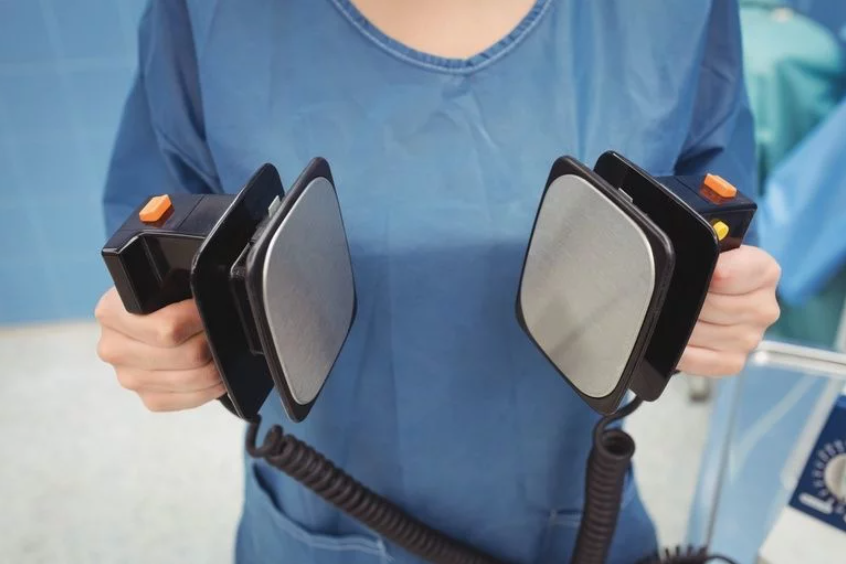
\includegraphics[width=6cm]{Bilder/defibrillator.png}
  \hspace{0.6cm}
  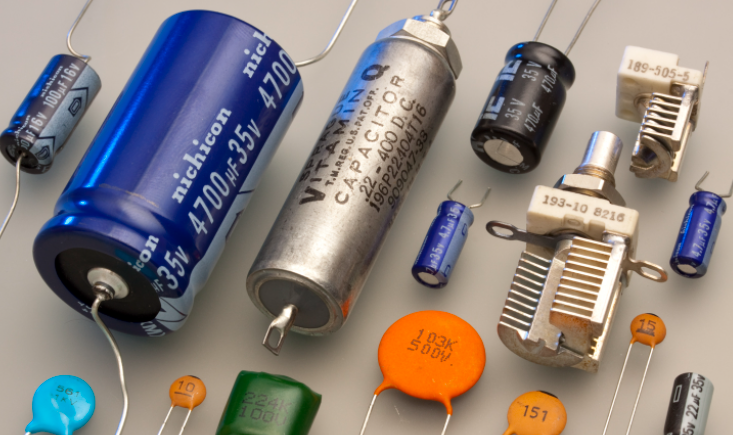
\includegraphics[width=6.7cm]{Bilder/kondensatoren.png}
\end{center}
{\scriptsize Links: Ein Defibrillator lädt sich langsam auf und gibt die
gespeicherte Ladung dann innert Millisekunden als kräftigen Stromstoss ab.
Rechts: Kondensatoren aus einem Elektronikladen, ganz unterschiedlich
gross und geformt.}
\end{beispielbox}

% =============================================================================
% Theorie 1: Was ist ein Kondensator? Die Batterie.
% =============================================================================
\begin{theoriebox}[Der Kondensator]
\begin{center}
\begin{tikzpicture}[>=Latex,scale=2]
  % Platten
  \draw[very thick] (0,-1.5) -- (0,1.5);
  \draw[very thick] (2.6,-1.5) -- (2.6,1.5);
  % Ladungen
  \foreach \y in {-1.1,-0.55,0,0.55,1.1} {
    \node at (-0.2,\y) {$+$};
    \node at (2.8,\y) {$-$};
  }
  % Feldlinien
  \foreach \y in {-0.9,-0.45,0,0.45,0.9} {
    \draw[->,accentblue] (0.15,\y) -- (2.45,\y);
  }
  % Abstand d
  \draw[<->] (0,-1.9) -- (2.6,-1.9) node[midway,below] {$d$};
  \node[accentblue] at (1.3,1.85) {$\vec{E}$};
\end{tikzpicture}
\hspace{1.2cm}
\begin{circuitikz}[scale=2.1]
  \draw (0,0) to[capacitor,l=$C$] (2,0);
\end{circuitikz}
\end{center}
{\scriptsize Links: Plattenkondensator im Querschnitt, mit homogenem
elektrischem Feld $\vec E$ zwischen den Platten. Rechts: Schaltzeichen für
einen Kondensator.}

\[
  \boxed{U = E\cdot d}
\]

\begin{center}
  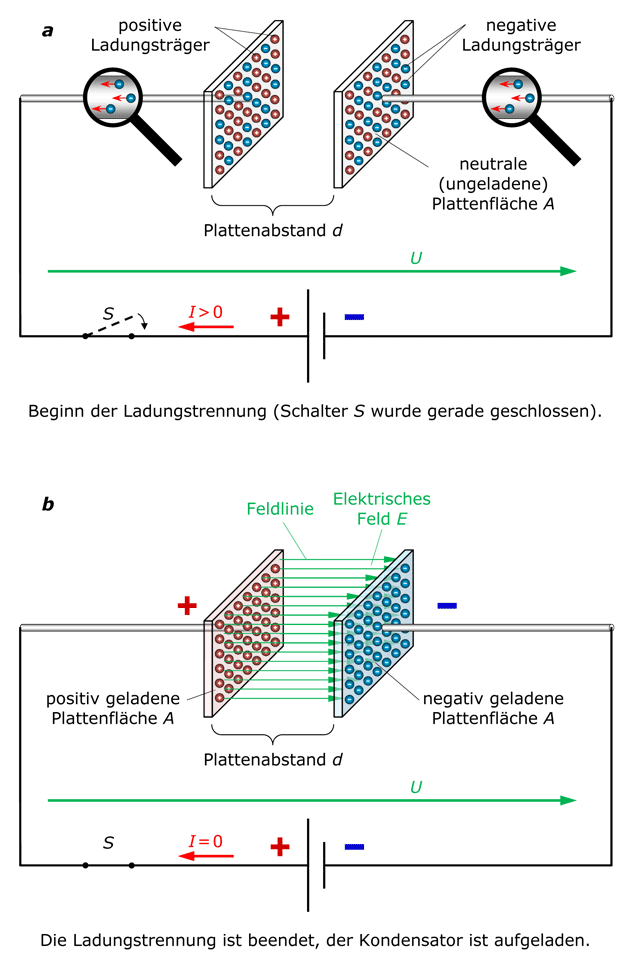
\includegraphics[width=7cm]{Bilder/Kondensator_aufladen.png}
\end{center}
{\scriptsize (a) Beginn der Ladungstrennung: Schalter $S$ wurde gerade
geschlossen, es fliesst ein Strom $I>0$, die Platten sind noch neutral.
(b) Die Ladungstrennung ist beendet, der Kondensator ist aufgeladen: Es
fliesst kein Strom mehr ($I=0$), zwischen den Platten liegt das Feld
$\vec E$.}
\end{theoriebox}

% =============================================================================
% Plenum 1: Q-U-Diagramm, Definition der Kapazität
% =============================================================================
\begin{questions}
\begin{groupbox}[Plenum: Kondensatoren im Vergleich]
Sie haben in der Lernaufgabe bereits selbst gemessen, wie $Q$ von $U$
abhängt. Vergleichen Sie nun im Plenum zwei Kondensatoren
unterschiedlicher Kapazität, die beide an dieselbe Batterie angeschlossen
werden (Spannung $U_0$).

\begin{center}
\begin{tikzpicture}[scale=2]
  \draw[-{Latex}] (0,0) -- (5.5,0) node[right] {$U$};
  \draw[-{Latex}] (0,0) -- (0,4.5) node[above] {$Q$};
  \draw[thick,accentblue] (0,0) -- (4.6,4.14);
  \node[accentblue,right] at (4.6,4.14) {$C_1$};
  \draw[thick,accentorange] (0,0) -- (4.6,2.3);
  \node[accentorange,right] at (4.6,2.3) {$C_2$};
  \draw[dashed] (3.2,0) -- (3.2,2.88);
  \draw[dashed] (3.2,2.88) -- (0,2.88);
  \draw[dashed] (3.2,1.6) -- (0,1.6);
  \filldraw (3.2,2.88) circle (1.3pt);
  \filldraw (3.2,1.6) circle (1.3pt);
  \node[below] at (3.2,0) {$U_0$};
  \node[left] at (0,2.88) {$Q_1$};
  \node[left] at (0,1.6) {$Q_2$};
\end{tikzpicture}
\end{center}
{\scriptsize Bei derselben Spannung $U_0$ speichert der Kondensator mit
der steileren Gerade ($C_1$) mehr Ladung als jener mit $C_2$.}

\question[2] Erklären Sie den Unterschied zwischen den beiden
Kondensatoren im Diagramm, und notieren Sie die daraus folgende
Definitionsgleichung für die Kapazität $C$.
\Antwortraum{2}
\begin{solution}
Bei derselben Spannung $U_0$ speichert der Kondensator mit der steileren
Gerade ($C_1$) mehr Ladung: $Q$ ist proportional zu $U$, und die Steigung
der jeweiligen Gerade entspricht der Kapazität. Im Plenum daraus
hergeleitete Definitionsgleichung:
\[
  \boxed{C := \frac{Q}{U}}, \qquad [C] = 1\ \frac{\text{C}}{\text{V}} = 1\ \text{Farad} = \SI{1}{\farad}.
\]
\end{solution}

In der Praxis sind Kapazitäten oft winzig, deshalb meist mit Präfix
angegeben:
\[
  \SI{1}{\pico\farad} = \SI{e-12}{\farad}, \quad
  \SI{1}{\nano\farad} = \SI{e-9}{\farad}, \quad
  \SI{1}{\micro\farad} = \SI{e-6}{\farad}, \quad
  \SI{1}{\milli\farad} = \SI{e-3}{\farad}.
\]
\end{groupbox}
\end{questions}

% =============================================================================
% Theorie 1b: Die Wassertankanalogie
% =============================================================================
\begin{theoriebox}[Die Wassertankanalogie]
\begin{center}
  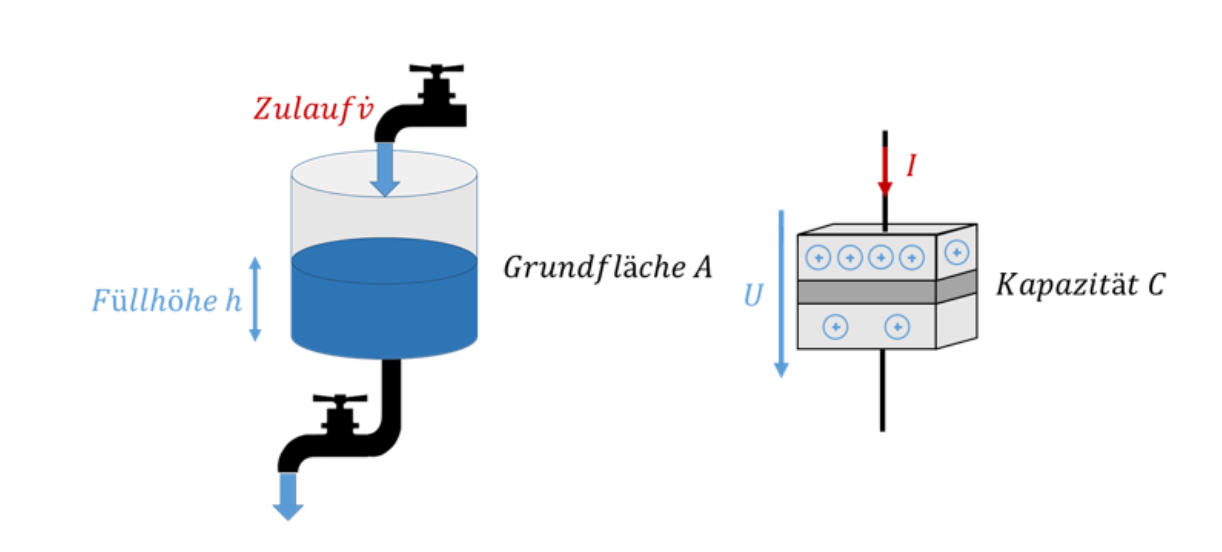
\includegraphics[width=9cm]{Bilder/wasserfass-vs-kondensator.png}
\end{center}
{\scriptsize Ein Wassertank als mechanische Analogie zu einem
Kondensator.}

\begin{center}
  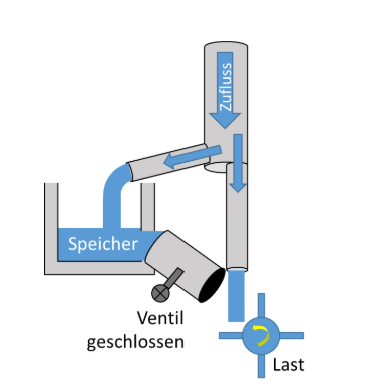
\includegraphics[width=5.5cm]{Bilder/wassertank_ventil_zu.png}
  \hspace{0.6cm}
  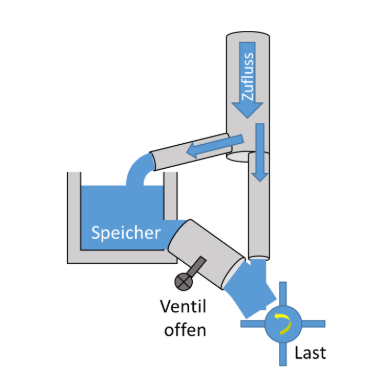
\includegraphics[width=5.5cm]{Bilder/wassertank_ventil_offen.png}
\end{center}
{\scriptsize Links: Ventil geschlossen, nur die Hauptleitung versorgt die
Last. Rechts: Ventil geöffnet, der Speicher liefert zusätzliches Wasser.}

\textbf{Sortieraufgabe (Partnerarbeit):}
\begin{questions}
\question[5] Ordnen Sie zu zweit die Grössen des Wassertanks (links) den
entsprechenden Grössen des Kondensators (rechts) zu, indem Sie sie mit dem
Stift verbinden.

\begin{center}
\renewcommand{\arraystretch}{1.3}
\begin{tabular}{>{\raggedleft\arraybackslash}p{5.2cm}c@{\hspace{2.2cm}}cP{5.2cm}}
1. Grundfläche $A_{\text{Tank}}$ des Tanks & $\bullet$ & $\bullet$ & A. Ladung $Q$ \\
2. Füllstand $h$ (Wasserspiegelhöhe) & $\bullet$ & $\bullet$ & B. Kapazität $C$ \\
3. Wassermenge im Tank & $\bullet$ & $\bullet$ & C. Spannung $U$ \\
4. Maximales Volumen $V_{\max}=A_{\text{Tank}}\cdot h_{\max}$ & $\bullet$ & $\bullet$ & D. Lade-/Entladestrom \\
5. Zu-/Abfluss von Wasser & $\bullet$ & $\bullet$ & E. Maximale Ladung $Q_{\max}=C\cdot U_{\max}$ \\
\end{tabular}
\renewcommand{\arraystretch}{1}
\end{center}

\begin{solution}
1 passt zu B, 2 passt zu C, 3 passt zu A, 4 passt zu E, 5 passt zu D.
\end{solution}
\end{questions}

\textbf{Frage:} Welche Rolle könnte ein Kondensator wohl in einem
Stromkreis spielen?
\Antwortraum{2}
\begin{solution}
Reicht die Batterie (Hauptleitung) allein nicht für einen kurzfristig
hohen Bedarf, liefert ein zuvor aufgeladener Kondensator (Speicher)
zusätzlich Ladung, bis er entladen ist -- genau wie beim Defibrillator aus
dem Einstieg.
\end{solution}
\end{theoriebox}

% =============================================================================
% Theorie 2: Kapazität und Kondensatorformel
% =============================================================================
\begin{theoriebox}[Kapazität und Plattengeometrie: die bekannten Bausteine]
\textbf{Repetition:} Aus der Elektrostatik wissen Sie bereits, dass die
elektrische Feldstärke einer geladenen Platte
$E=\frac{Q}{2\varepsilon_0\cdot A}$ beträgt, und dass sich zwischen zwei
Platten eines Plattenkondensators die Feldstärke verdoppelt:
\[
  \boxed{E = \frac{Q}{\varepsilon_0\cdot A}} \qquad \text{(zwischen den Platten, Randeffekte vernachlässigt)},
  \qquad [E] = \si{\volt\per\meter}.
\]
mit $\varepsilon_0\approx\SI{8.85e-12}{\farad\per\meter}$, der bereits aus
der Coulombkraft bekannten elektrischen Feldkonstante, und $A$: Plattenfläche
(Einheit \si{\meter\squared}). Ausserhalb der Platten gilt $E\approx0$.

Ebenfalls aus der Elektrostatik bereits bekannt: Für die Spannung zwischen
den Platten gilt
\[
  \boxed{U = E\cdot d}, \qquad [U] = \si{\volt}
\]
($d$: Plattenabstand, Einheit \si{\meter}).

\begin{hinweisbox}[Zu beachten: Das Feld im Plattenkondensator ist konstant]
Im Gegensatz zum Feld einer einzelnen Punktladung, das mit dem Abstand
abnimmt, ist das elektrische Feld \textbf{\emph{zwischen den Platten eines
Plattenkondensators überall gleich gross}} (homogenes Feld), unabhängig
davon, wie nahe man sich an welcher Platte befindet. Diese Eigenschaft
haben wir bereits in der Elektrostatikeinheit hergeleitet und benutzen sie
hier direkt weiter.
\end{hinweisbox}
\end{theoriebox}

% =============================================================================
% Plenum 2: Von der Geometrie zur Kondensatorformel
% =============================================================================
\begin{questions}
\begin{groupbox}[Plenum: Von der Geometrie zur Kondensatorformel]
Die nächste Simulationsansicht zeigt direkt die Kapazität eines
Plattenkondensators. Sie kennen bereits drei Formeln:
\[
  E = \frac{Q}{\varepsilon_0\cdot A}, \qquad U = E\cdot d, \qquad C = \frac{Q}{U}.
\]

\needspace{12cm}
\question[4] Kombinieren Sie diese drei Formeln im Plenum, um eine Formel
für die Kapazität $C$ eines Plattenkondensators zu finden. Zeigen Sie
Ihren Rechenweg.
\Antwortraum{4}
\begin{solution}
$E=\dfrac{Q}{\varepsilon_0\cdot A}$ in $U=E\cdot d$ eingesetzt:
\[
  U = \frac{Q}{\varepsilon_0\cdot A}\cdot d.
\]
Mit $\varepsilon_0\cdot A$ multiplizieren:
\[
  U\cdot\varepsilon_0\cdot A = Q\cdot d.
\]
Durch $d$ dividieren, nach $Q$ aufgelöst:
\[
  Q = U\cdot\frac{\varepsilon_0\cdot A}{d}.
\]
Vergleich mit $Q=C\cdot U$: Der Vorfaktor von $U$ muss die Kapazität sein:
\[
  \boxed{C = \frac{\varepsilon_0\cdot A}{d}}.
\]
\end{solution}
\end{groupbox}
\end{questions}

% =============================================================================
% Experiment
% =============================================================================
\begin{questions}
\begin{groupbox}[Experiment: Kondensator und Lichtquelle]
\question[3] Kommen Sie nach vorne: Kondensatoren unterschiedlicher
Kapazität werden nacheinander an einer Spannungsquelle aufgeladen, danach
an eine kleine Lichtquelle angeschlossen.

\begin{center}
\begin{minipage}[c]{4.6cm}
  \centering
  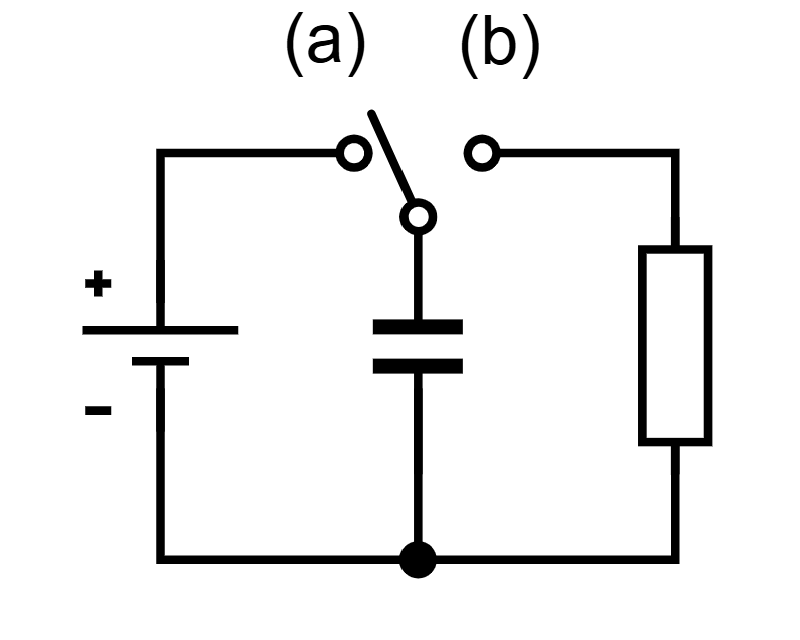
\includegraphics[width=4.5cm]{Bilder/Kondensator_stromkreis.png}
\end{minipage}%
\hspace{0.6cm}
\begin{minipage}[c]{5.3cm}
  \centering
  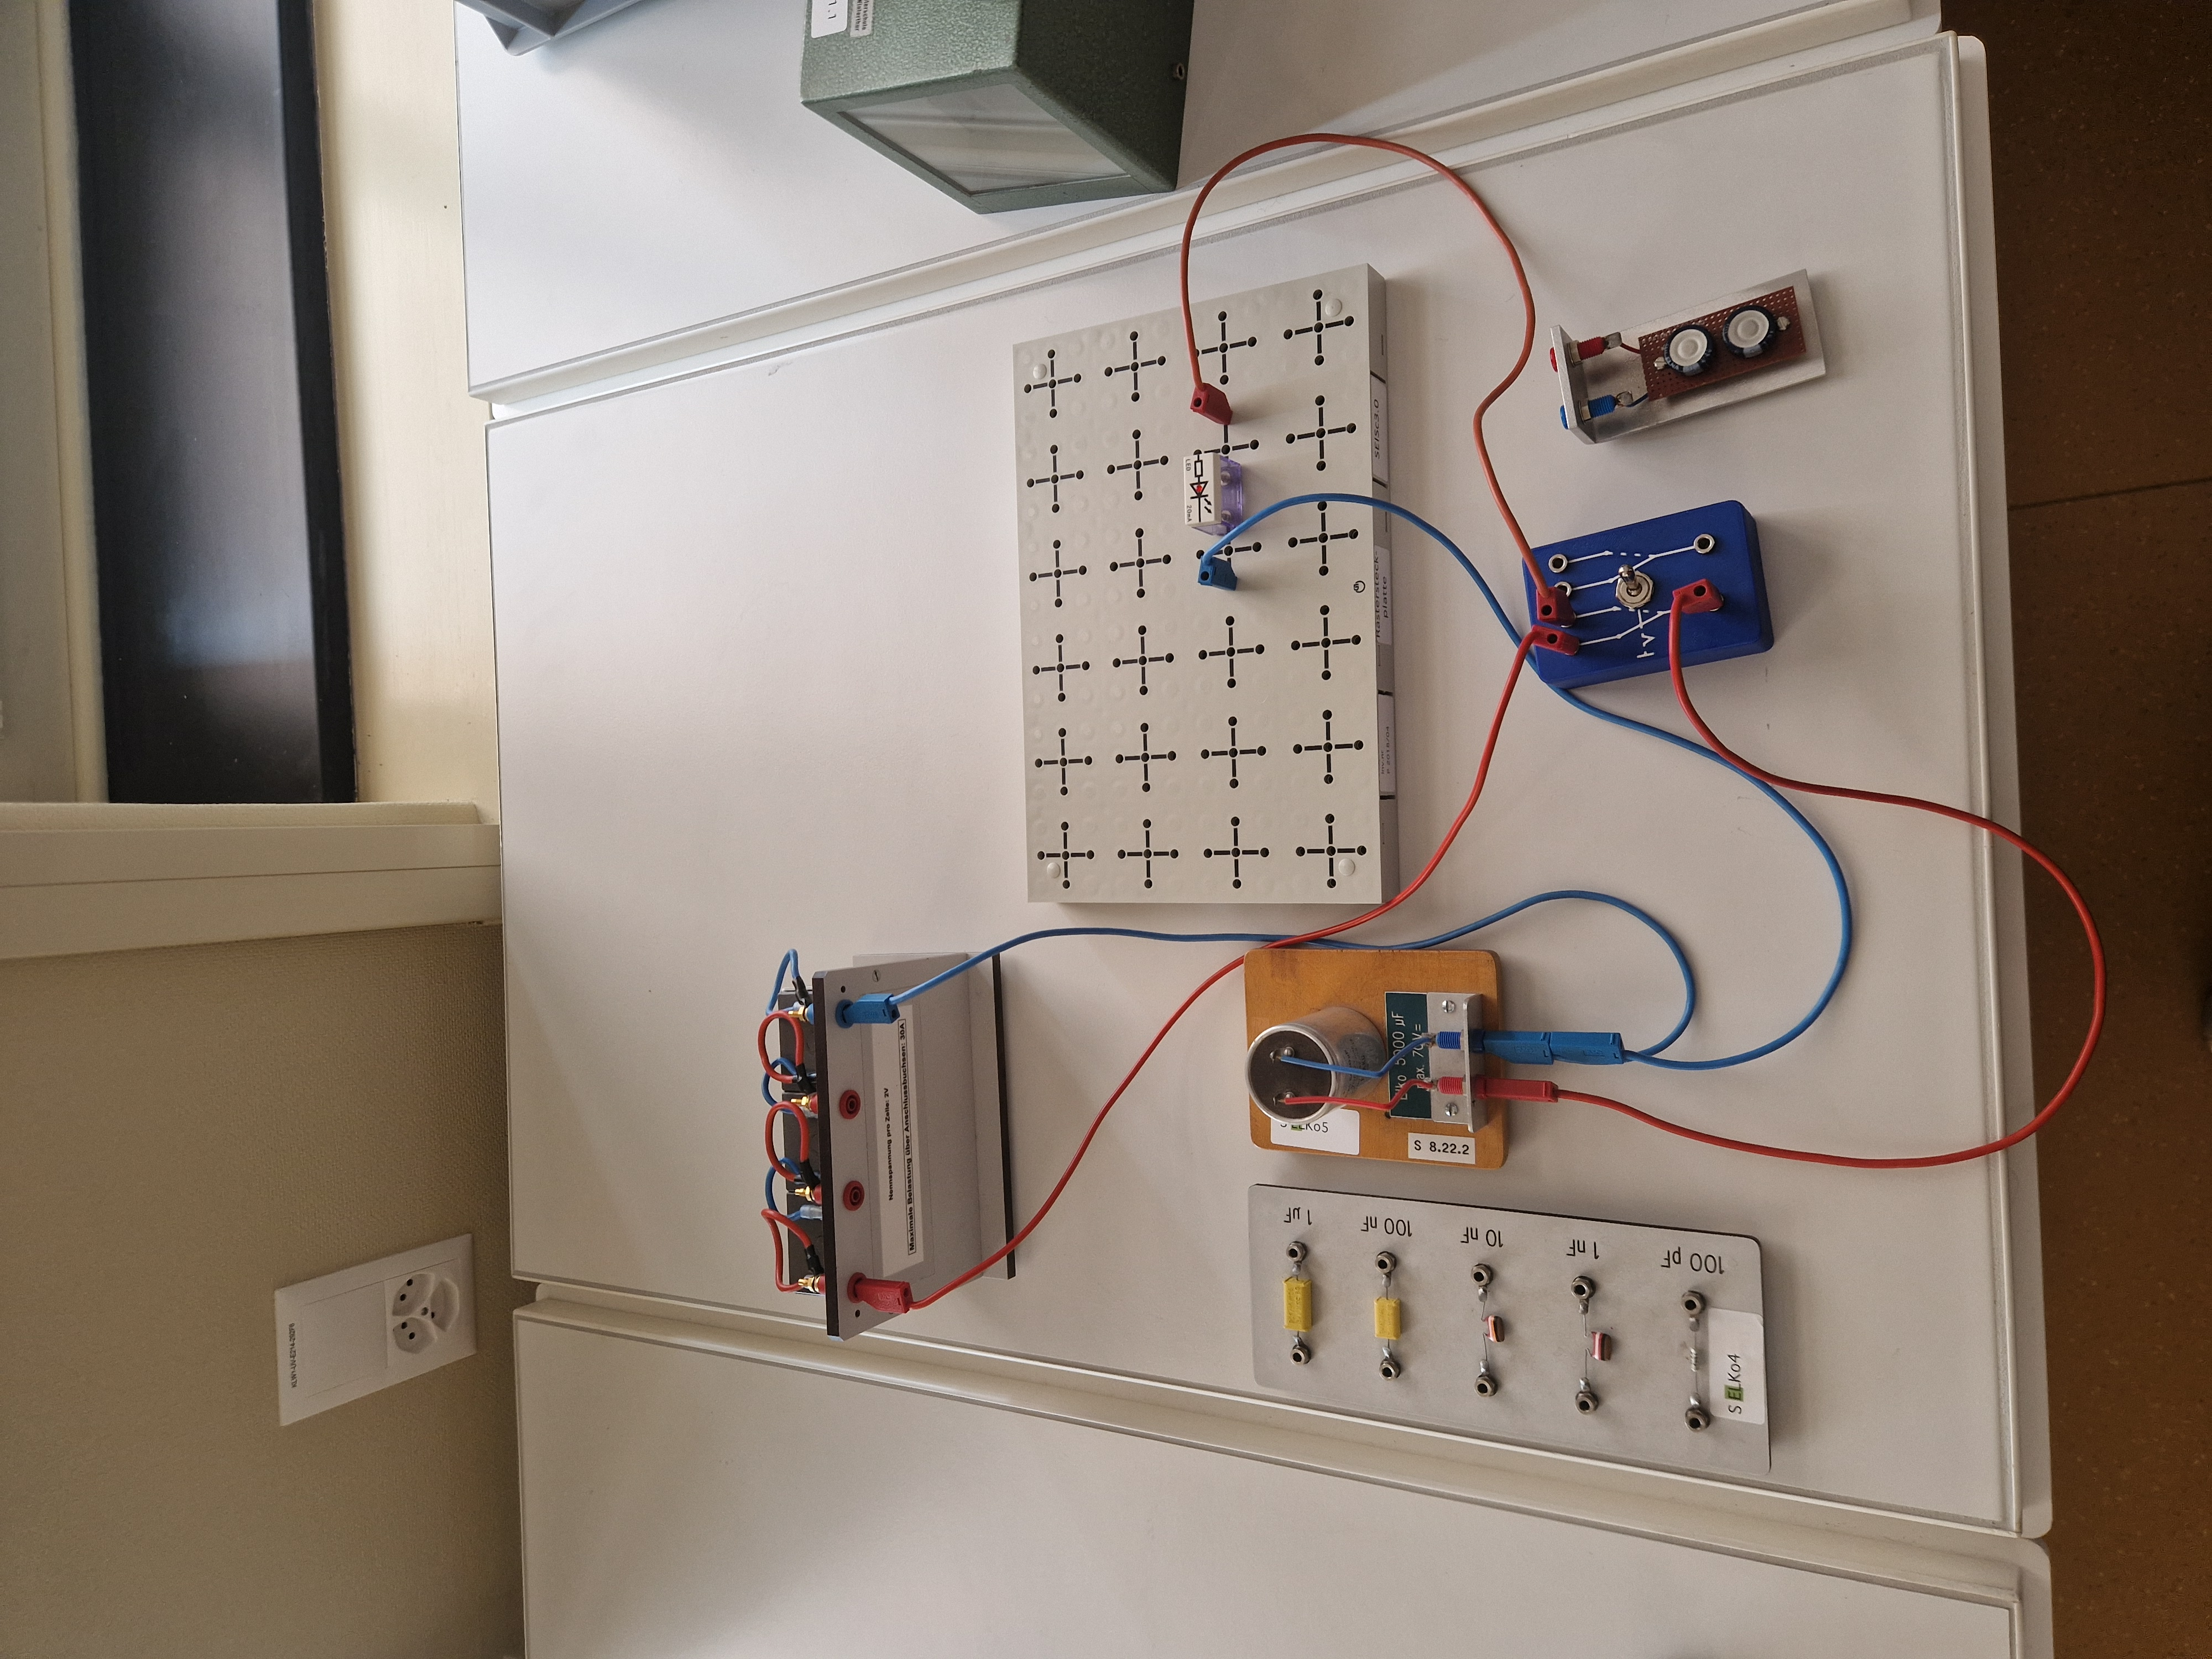
\includegraphics[width=5.2cm,angle=-90]{Bilder/Kapazitäten_Experiment.jpg}
\end{minipage}
\end{center}
{\scriptsize Links: Schaltschema -- Schalter (a) lädt den Kondensator an
der Spannungsquelle, Schalter (b) verbindet ihn danach mit der
Lichtquelle. Rechts: Versuchsaufbau mit verschiedenen Kondensatoren
(100\,pF bis 1\,\textmu F), Spannungsquelle, Schalter und Lichtquelle
(LED).}

Leuchtet die Lichtquelle bei allen Kondensatoren gleich lange? Begründen
Sie Ihre Vorhersage mit der Wassertankanalogie, bevor Sie den Versuch
beobachten.
\Antwortraum{3}

\begin{solution}
Ein Kondensator mit grösserer Kapazität kann bei gleicher Spannung mehr
Ladung speichern, analog zu einem Wassertank mit grösserer Grundfläche, der
bei gleichem Füllstand mehr Wasser enthält. Die Lichtquelle leuchtet
deshalb bei grösserer Kapazität länger.
\end{solution}
\end{groupbox}
\end{questions}

% =============================================================================
% Theorie 3: Das Dielektrikum
% =============================================================================
\begin{theoriebox}[Das Dielektrikum]
\begin{center}
  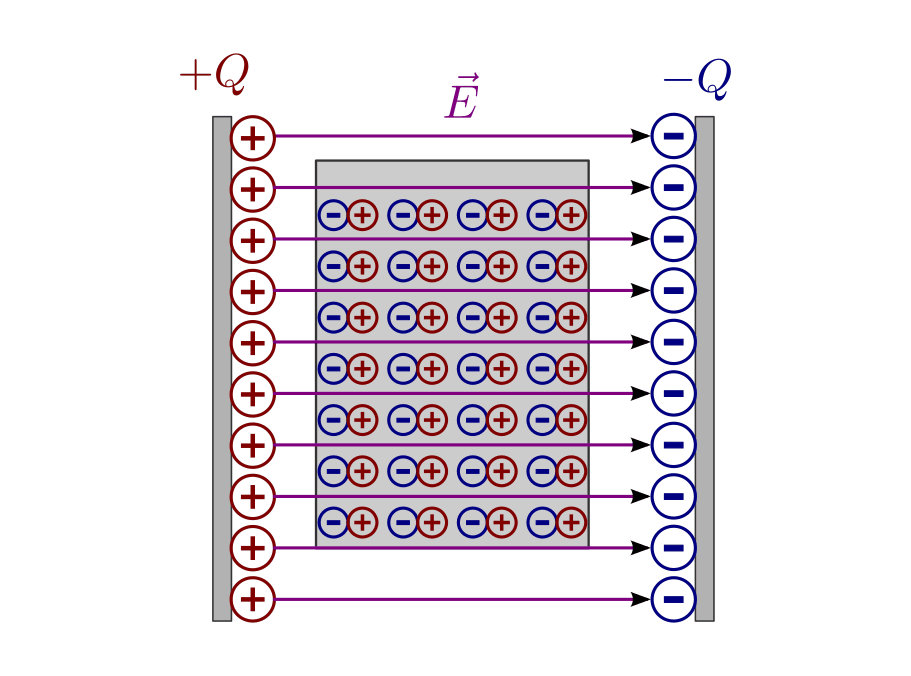
\includegraphics[width=7.5cm]{Bilder/plattenkondensator-polarisation.png}
  \hspace{0.5cm}
  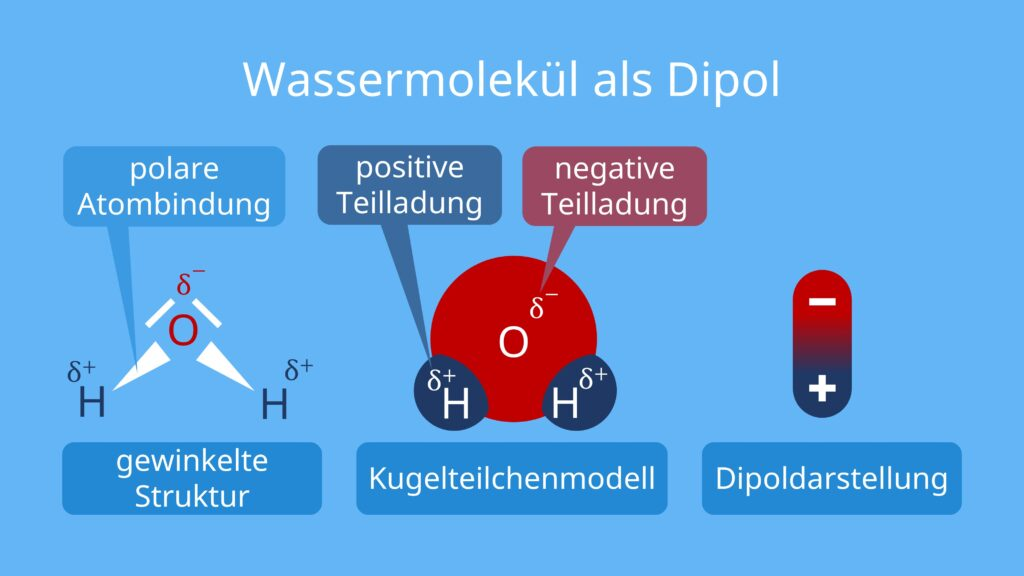
\includegraphics[width=6cm]{Bilder/03_Wassermolekül-als-Dipol-1024x576.jpg}
\end{center}
{\scriptsize Links: Die Moleküle im Dielektrikum richten sich im Feld
$\vec E$ aus (\textbf{\emph{Polarisation}}), jeweils als kleiner Dipol
dargestellt. Rechts: Ein Wassermolekül ist bereits von sich aus ein Dipol.
Deshalb hat Wasser eine besonders hohe relative Permittivität
$\varepsilon_r\approx80$ (Porzellan zum Vergleich nur $\varepsilon_r\approx7$).}

\begin{center}
  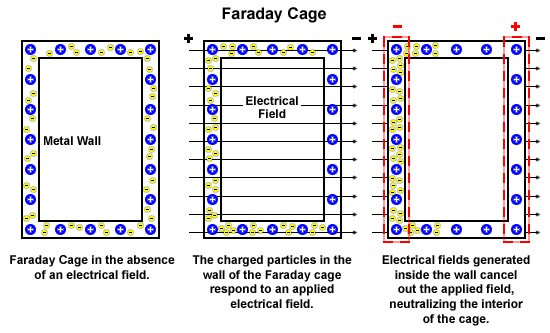
\includegraphics[width=9cm]{Bilder/faraday_kaefig.jpg}
\end{center}
{\scriptsize Faraday-Käfig: Influenzierte Ladungen in der Wand heben das
Feld im Innern auf.}
\end{theoriebox}

% =============================================================================
% Anwendung: Kapazitive Sensoren (Kofferraumsensor, Touchscreen)
% =============================================================================
\begin{beispielbox}[Anwendung: Kapazitive Sensoren]
Menschliches Gewebe hat wegen seines hohen Wassergehalts eine grosse
relative Permittivität $\varepsilon_r$ (siehe oben) und wirkt deshalb
selbst wie ein Dielektrikum. Nähert sich ein Körperteil einer
Kondensatorplatte, steigt dadurch die gemessene Kapazität messbar an.
Genau das nutzen kapazitive Sensoren aus.

\begin{center}
  
\includegraphics[width=4.2cm]{Bilder/autosensor.png}
  \hspace{0.4cm}
  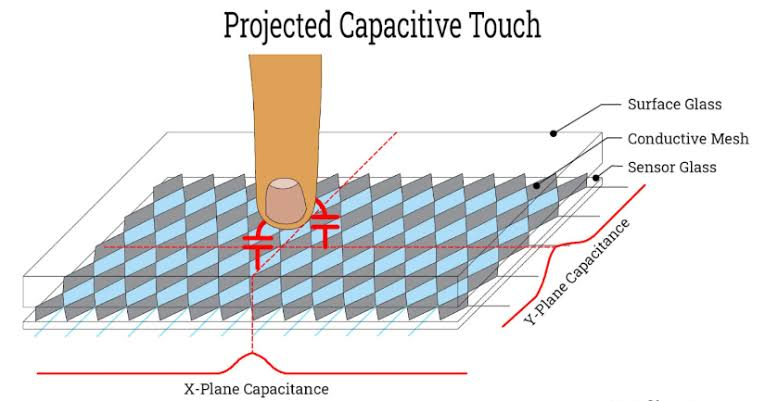
\includegraphics[width=4.6cm]{Bilder/touchscreen.jpg}
  \hspace{0.4cm}
  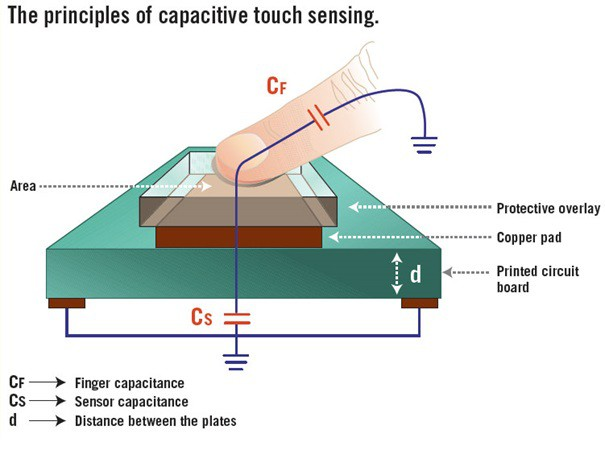
\includegraphics[width=4.6cm]{Bilder/touchscreen_parallel_capacitance.jpg}
\end{center}
{\scriptsize Links: Kapazitiver Kofferraumsensor. Eine Fussbewegung
unter der Stossstange ändert die Kapazität der Sensorelektrode und löst
das Öffnen aus. Mitte: Kapazitiver Touchscreen. Der Finger ändert die
Kapazität an den Kreuzungen des Elektrodengitters (rote
Kondensatorsymbole). Rechts: Ersatzschaltbild dazu. Der Finger bildet
mit der Elektrode einen zusätzlichen Kondensator $C_F$, parallel zur
Sensorkapazität $C_S$.}

Beim \textbf{\emph{Kofferraumsensor}} mancher Autos genügt eine
Fussbewegung unter der Stossstange, um die Klappe zu öffnen: Der Fuss
verändert die Kapazität einer dort verbauten Elektrode, der Sensor
erkennt die Änderung und löst aus. Der \textbf{\emph{Touchscreen}} Ihres
Smartphones funktioniert nach demselben Prinzip, nur mit dem Finger auf
einem Gitter aus vielen kleinen Elektroden.
\end{beispielbox}

% =============================================================================
% Herleitung: Kapazität mit Dielektrikum
% =============================================================================
\begin{questions}
\begin{groupbox}[Herleitung (Partnerarbeit): Kapazität mit Dielektrikum]
\question Der Kondensator bleibt während des ganzen Vorgangs an einer
Batterie angeschlossen, die eine \textbf{konstante Spannung $U$} liefert;
der Plattenabstand $d$ bleibt ebenfalls unverändert.

\begin{center}
  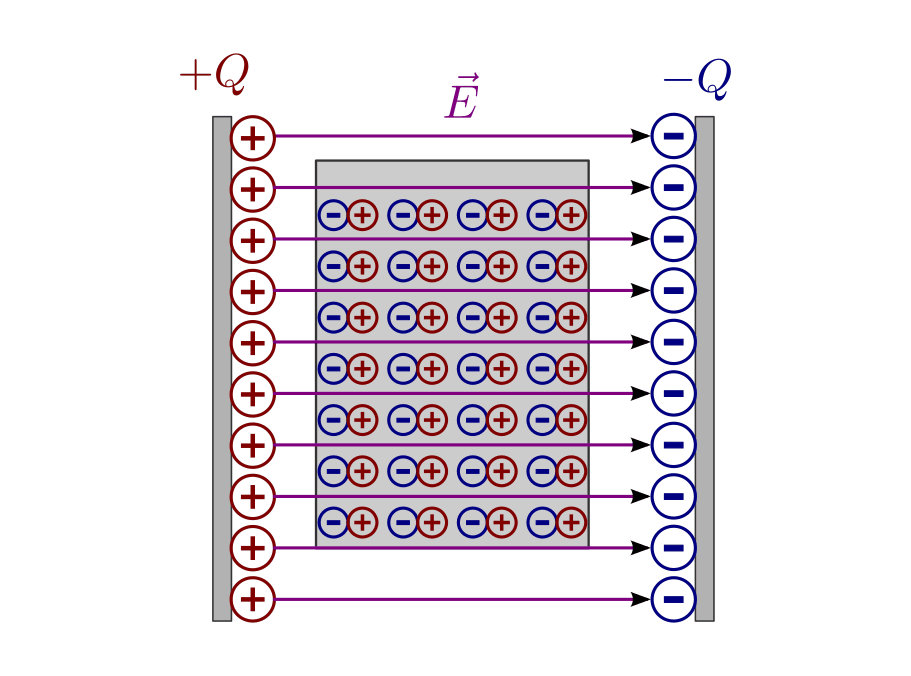
\includegraphics[width=9cm]{Bilder/plattenkondensator-polarisation.png}
\end{center}
{\scriptsize Die Moleküle im Dielektrikum richten sich im Feld $\vec E$
aus (\textbf{\emph{Polarisation}}), jeweils als kleiner Dipol dargestellt.}

\begin{hinweisbox}[Tipp]
Ein elektrisches Feld entsteht durch Ladungen. Überlegen Sie: Was passiert
mit den Ladungen der einzelnen Dipole \emph{im Inneren} des Dielektrikums,
und was mit denen ganz \emph{am Rand}?
\end{hinweisbox}
\begin{parts}
  \part[3] Ergänzen Sie das Bild aus der Theorie: Skizzieren Sie den
  Plattenkondensator mit dem polarisierten Dielektrikum, und zeichnen Sie
  ein, wo im Material eine Nettoladung übrig bleibt und weshalb.
  Zeichnen Sie zusätzlich das dadurch entstehende Polarisationsfeld
  $E_{\text{pol}}$ ein.
  \begin{answerbox}
    \rule{0pt}{6.5cm}
  \end{answerbox}
  \begin{solution}
  \begin{center}
    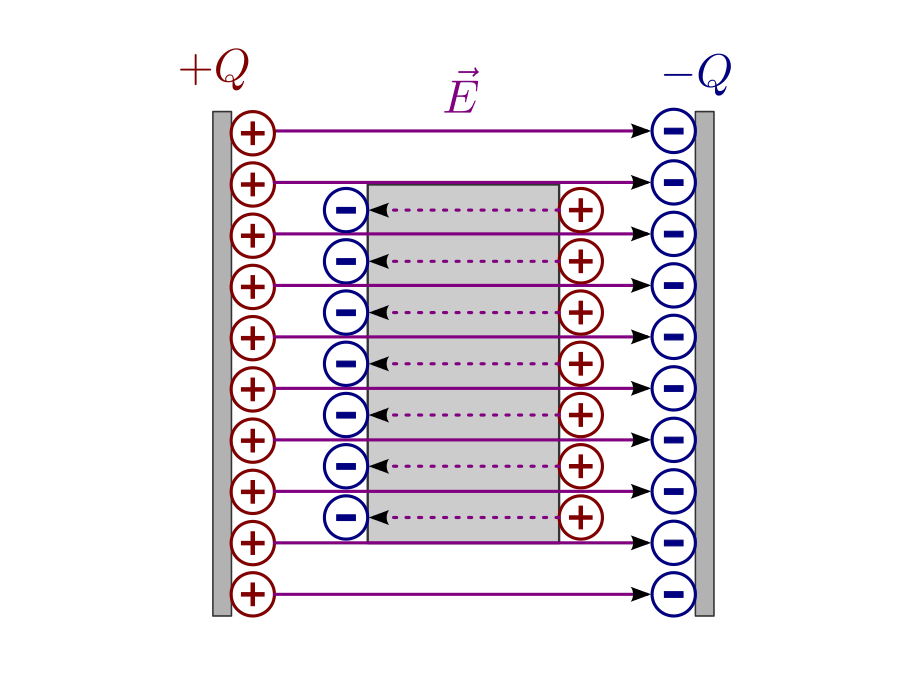
\includegraphics[width=6.2cm]{Bilder/plattenkondensator-influenz.png}
  \end{center}
  Im Inneren des Dielektrikums liegt neben der positiven Seite eines
  Dipols immer die negative Seite des Nachbardipols: Diese Ladungen heben
  sich gegenseitig auf. Nur an den beiden äusseren Rändern des
  Dielektrikums gibt es keinen Nachbardipol zum Ausgleich: Dort bleibt
  eine Nettoladung übrig, negativ auf der Seite der $+Q$-Platte und
  positiv auf der Seite der $-Q$-Platte. Diese Randladung erzeugt das
  eingezeichnete Polarisationsfeld $E_{\text{pol}}$, das dem äusseren
  Feld entgegengerichtet ist.
  \end{solution}

  \part[2] Was bedeutet das für das Gesamtfeld $E$ zwischen den Platten?
  (Tipp: $U=E\cdot d$.)
  \Antwortraum{2}
  \begin{solution}
  Da $U$ und $d$ beide unverändert bleiben, bleibt auch $E=U/d$
  unverändert: Das Gesamtfeld ändert sich nicht.
  \end{solution}

  \part[3] Das Gesamtfeld setzt sich zusammen aus dem Feld der freien
  Ladung, $E_{\text{frei}}=Q/(\varepsilon_0\cdot A)$, und dem
  entgegengerichteten Polarisationsfeld: $E=E_{\text{frei}}-E_{\text{pol}}$.
  Nun ist $E_{\text{pol}}\neq0$ hinzugekommen, während $E$ nach
  Teilaufgabe (b) gleich gross bleiben muss. Was folgt daraus für
  $E_{\text{frei}}$ und damit für die freie Ladung $Q$ auf den Platten? Wie
  reagiert die Batterie darauf?
  \Antwortraum{3}
  \begin{solution}
  Das neu entstandene Polarisationsfeld $E_{\text{pol}}$ ist dem
  ursprünglichen Feld entgegengerichtet: Ohne Ausgleich würde das
  Gesamtfeld dadurch kleiner werden. Weil die Batterie das Feld $E$ nach
  Teilaufgabe (b) aber konstant hält, gleicht sie diese Schwächung sofort
  aus, indem sie zusätzliche freie Ladung auf die Platten schickt. Das
  geschieht so lange, bis das ursprüngliche Feld wieder erreicht ist. Die freie Ladung
  $Q$ auf den Platten nimmt dadurch zu.
  \end{solution}

  \part[1] Was folgt daraus für die Kapazität $C=Q/U$?
  \Antwortraum{1}
  \begin{solution}
  Da $Q$ zugenommen hat und $U$ gleich geblieben ist, muss $C=Q/U$
  zunehmen: Die Kapazität steigt.
  \end{solution}

  \needspace{8cm}
  \part[2] Definiert man die relative Permittivität als das Verhältnis der
  neuen zur ursprünglichen Kapazität, $\varepsilon_r:=C/C_0$, leiten Sie
  damit und mit der bereits bekannten Formel $C_0=\varepsilon_0\cdot A/d$
  (ohne Dielektrikum) die Formel für die Kapazität $C$ mit Dielektrikum
  her.
  \Antwortraum{2}
  \begin{solution}
  \[
    \varepsilon_r = \frac{C}{C_0} \quad\Longrightarrow\quad
    C = \varepsilon_r\cdot C_0 = \varepsilon_r\cdot\varepsilon_0\cdot\frac{A}{d}.
  \]
  \[
    \boxed{C = \varepsilon_r\cdot\varepsilon_0\cdot\frac{A}{d}}
  \]
  \end{solution}
\end{parts}
\end{groupbox}
\end{questions}

\end{document}
